\chapter{Beamforming}
\label{chapter:beamforming}
\chaptermark{Beamforming}

% ================================================================================
% CHAPTER OVERVIEW
% ================================================================================

% ======= Liam Notes  ========

% Need to discuss interferometry in the introduction,
% I think.

\section{Chapter Overview}

This chapter outlines the basic theory behind 
digital beamforming, and describes the commissioning 
of the first beamformer on CHIME Pathfinder. This 
includes the synthesis of several different software packages, 
the implementation of a scheduler, 
and an automated point-source calibration daemon that 
removes drifting instrumental gains in real-time. We will 
also detail early pulsar work and the beamformer's first light. 
Finally, the creation of an ongoing VLBI FRB search between 
the DRAO and ARO will be outlined, including early results. 
% ================================================================================
% INTRODUCTION
% ================================================================================

\section{Introduction}

Beamforming is a signal processing technique that allows for 
spatial filtering, and has greatly benefited a diverse set of fields 
from radar and wireless communications to radio astronomy 
\citep{1988IASSP...5....4V}. Whether being used in phased-array RADAR
\citep{2007BAMS...88.1753Z}, 
ultrasonic imaging \citep{macovski1983medical}, or 
wide-band radio astronomy \citep{2013PASA...30....7T}, beamforming 
allows for heightened sensitivity or output to select spatial
modes. This usually involves a sensor (in our case an antenna)
being used alongside a processor (in our case, a computing cluster) 
\citep{1988IASSP...5....4V}. Modern astronomy will benefit greatly from this
technology. 
Beamforming is particularly essential to CHIME. 
The pulsar back-end will rely on
brute-force beamforming in order to track ten sources at a time, 24-7.  
The FRB experiment will FFT-beamform to generate 1024 fan-beams, 
in order to search them in real time for radio transients. Finally, the cosmology 
experiment has always left itself the option of beamforming, whose 
computing cost scales as $N\log N$, as 
an alternative to the full $N^2$ correlation.
  
% ================================================================================
% THEORY AND IMPLEMENTATION
% ================================================================================
  
\section{Theory and Implementation}
\label{sec:theory}

By coherently combining the voltages of a multi-element array, 
sensitivity can be allocated to small regions of the sky and 
the array's effective forward gain can be increased. The signal 
from each antenna, $x_n$, is multiplied by a complex weight whose 
phases, $\phi_{n}$, are chosen a priori to maximally destructively interfere radio waves 
in all directions but the desired pointing. After applying 
such weights, the signals 
from all antennas are combined to give the formed-beam 
voltage stream, $X_{\rm BF}$.

\begin{equation}
\label{eq-bf_sum}
X_{\rm BF} = \sum_{{n}=1}^N a_n e^{i\phi_{n}} x_n
\end{equation}

\noindent Here $a_n$ are real numbers that can be used as 
amplitude weightings for the antennas. If we define a more 
general complex weighting, $w_n \equiv a_n e^{i\phi_{n}}$, and 
switch to vector notation, Eq.~\ref{eq-bf_sum} becomes,

\begin{equation}
X_{\rm BF} = \mathbf{w} \, \mathbf{x}^{\rm T} .
\end{equation}

\noindent In general, $X_{\rm BF}$ and $\mathbf{x}^{\rm T}$ will be 
functions of time and frequency. This is also true for $\mathbf{w}$,
unless one needs a static, non-tracking beam -- which is the case for the 
CHIME Pathfinder's transient search, described in
Sect.~\ref{vlbi_frb}. We can write this explicitly as follows,


\begin{align}
     \mathbf{w}_{\rm t \nu} &= \left (a_1(\nu) e^{i \phi_1(\nu)}, \, 
     a_2(\nu) e^{i \phi_2(\nu)}, ... \,, \,a_N(\nu) e^{i \phi_N(\nu)} \right )\\
     \mathbf{x}_{\rm t \nu} &= \left ( x_1(\rm{t}, \nu), \, x_2(\rm{t}, \nu), 
     ..., \, x_N(\rm{t}, \nu) \right ).
\end{align}

The voltage stream, $X_{\rm BF}$, is then effectively squared and integrated 
to give a visibility stream. 
In the case of CHIME, $X_{\rm BF}$ corresponds to a single polarization 
so to get the full Stokes information one must compute the 
north-south polarization's autocorrelation, the east-west autocorrelation, 
and their cross-correlation. The Stokes vector can be written as,

% Make sure Stokes stuff is already defined.
\begin{equation}
\mathbf{S} = 
\begin{pmatrix}
I \\ 
Q \\ 
U\\ 
V
\end{pmatrix}
= \begin{pmatrix}
\, X_{\rm ew} X_{\rm ew}^* + X_{\rm ns} X_{\rm ns}^*\, \\ 
\, X_{\rm ew} X_{\rm ew}^* - X_{\rm ns} X_{\rm ns}^* \,\\ 
\, \Re e(X_{\rm ew} X_{\rm ns}^*)\,\\ 
\, \Im m(X_{\rm ew} X_{\rm ns}^*)\,
\end{pmatrix}.
\end{equation}


\subsection{Geometric phase}

We now need to calculate $\phi_n$ across the array.
Ignoring instrumental phases for now, one can compute the geometric 
phases for an antenna by projecting its position vector, $\mathbf{d}_n$, 
onto the pointing vector, $\hat{\mathbf{k}}$. This gives,

\begin{equation}
\label{eqn-phi_n}
\phi_n = \frac{2\pi}{\lambda} \, \mathbf{d}_n \cdot  {\mathbf{\hat{k}}},
\end{equation}

\noindent where we have taken $\mathbf{d}_n$ to be the baseline vector between 
feed $n$ and an arbitrary reference point, and $\phi_n$ is the corresponding 
phase difference. A sketch for this is shown in 
Fig.~\ref{fig-bf_diagram} on page 
\pageref{fig-bf_diagram}.


%trim={<left> <lower> <right> <upper>}
\begin{figure}[!h]
\label{fig-bf_diagram}
\begin{center}
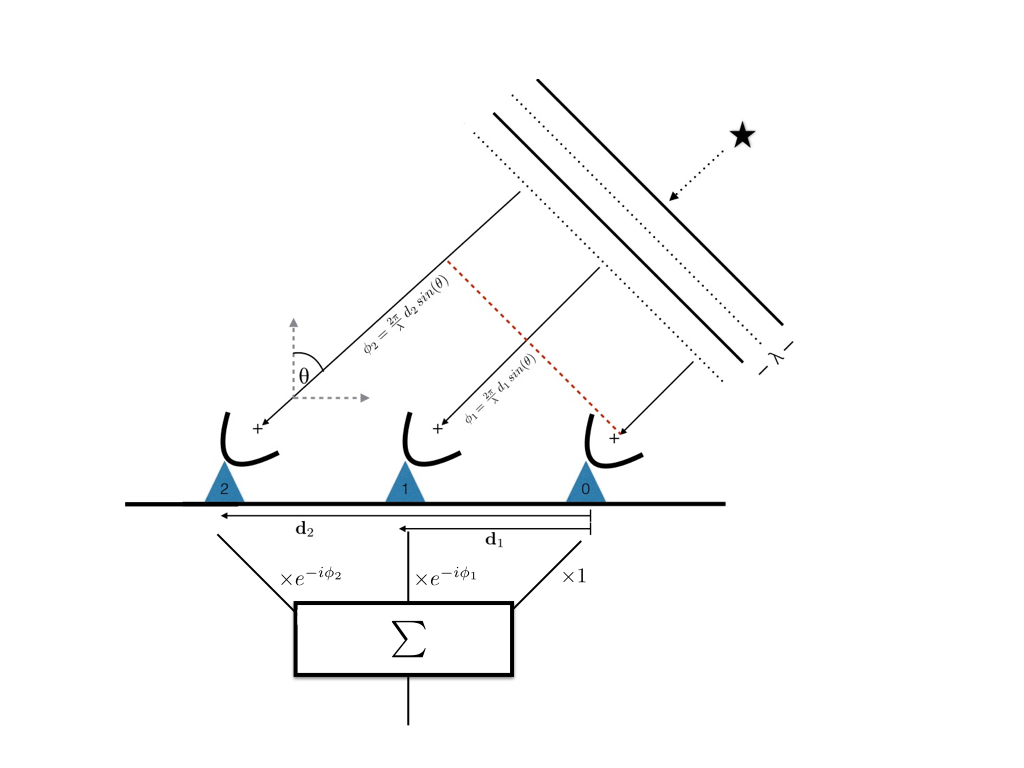
\includegraphics[trim={1.in, 1.in, 2.5in, 1.in}, width=1\textwidth]{./figures/beamforming/beamforming_diagram.jpeg} 
\vspace{0.0cm}
\caption[abc]{Diagrammatic example of a three-element beamformer. The 
wavefront from a far-field point-source arrives at each antenna 
at different times, but the delay is calculable given an array 
configuration and a direction to the object. Complex weights can 
be applied to each antenna's voltage time-stream to account 
for the geometric delay, allowing for the signals to be summed coherently.}  
\vspace{-0.4cm}   
\end{center}
\end{figure}

To calculate the projection $\mathbf{d}_n \cdot  {\mathbf{\hat{k}}}$, we 
need to go from celestial coordinates, in this case equatorial, to geographic 
coordinates. This requires only a source location, an observer location, and an 
observing time. For the latter we use local 
sidereal time (LST), which is the $RA$ of the local meridian. This can be determined  
by an observer's longitude and a time, e.g. a Coordinated Universal Time (UTC). 
A source's hour angle is simply the difference between $LST$ and its $RA$,

\begin{equation}
HA = LST - RA.
\end{equation}

We use the standard interferometric $(u, v, w)$ coordinate system 
to describe our baseline vector, $\mathbf{d}_n$. This is a 
right-handed coordinate system where $u$ (east-west) and $v$ (north-south) are in the plane 
whose normal is the zenith, and $w$ measures the vertical direction \citep{1986isra.book.....T}.
They are defined in numbers of wavelengths, with
$u = d_{\rm ew} / \lambda$, $v = d_{\rm ns} / \lambda$, 
and $w = d_{\rm vert} / \lambda$. Eq.~\ref{eqn-phi_n} can be expanded 
as,

\begin{align}   
\phi_n &= 2\pi \, (u, v, w) \cdot \mathbf{\hat{k}}\\
&= 2 \pi \left ( 
u \, \mathit{\mathbf{\hat{u}}} \cdot \mathbf{\hat{k}} + 
v \, \mathbf{\hat{v}} \cdot \mathbf{\hat{k}} + 
w \, \mathbf{\hat{w}} \cdot \mathbf{\hat{k}} 
\right ),
\end{align}

\noindent where each projection component can be obtained 
using spherical trigonometry. Though we do not go through the
derivation here, it is given by the following product,

\begin{equation}
\label{eq-fringestop_phase}
\mathbf{d}_n \cdot  {\mathbf{\hat{k}}} = \lambda \begin{pmatrix}
u, & v, & w
\end{pmatrix}  \cdot \begin{pmatrix} 
-\mathrm{cos}\delta \,\mathrm{sin}HA \\ 
\, \mathrm{cos}(lat) \, \mathrm{sin}\delta - \mathrm{sin}(lat) \, \mathrm{cos}\delta \, \mathrm{cos}HA \,\\
\, \mathrm{sin}(lat) \, \mathrm{sin}\delta + \mathrm{cos}(lat) \, \mathrm{cos}\delta \, \mathrm{cos} HA\,
\end{pmatrix} .
\end{equation}

These phases are not only essential to beamforming but 
also for the fringestopping process, which is ubiquitous in 
interferometric analysis and is descibed in Sect.~\ref{sec-instr_phases}.


\begin{table}[]
\centering
\label{tab-coord_var}
\begin{tabular}{ll}
\multicolumn{1}{c}{\textbf{Variable}} & \multicolumn{1}{c}{\textbf{Coordinate}} \\ \hline
$\delta$                              & Source declination                      \\
$RA$                                    & Source right ascention                  \\
$LST$                                   & Local sidereal time                     \\
$HA$                                    & Source hour angle                       \\
$alt$                                   & Source altitude                         \\
$az$                                    & Source azimuth                          \\
$lat$                                   & Telescope latitude                      \\
$lon$                                   & Telescope longitude                    
\end{tabular}
\end{table}

\section{Pathfinder beamformer}

\subsection{Instrumental phases}
\label{sec-instr_phases}
In a real experiment, if the voltages from each antenna, $x_n$, are summed 
without any adjustment from those written in Eq~\ref{eq-bf_sum}, one should only 
expect noise and not a coherent beam. This is because we have assumed 
the wavefront's differential time-of-arrival across at array 
is the same time delay seen by the correlator. In fact each 
signal is further delayed by multiple steps in the signal chain, 
often randomly. 
Digital phases in the electronics can be added by the LNAs and FLAs; 
coaxial cables, whose lengths vary by up to a meter, can rotate 
the signal by multiple radians. Therefore in order to coherently sum 
across the array and beamform, the instrumental phases must be removed. 
If $e_n$ is the true electric field on the 
sky as seen by each feed, then the thing we measure is the on-sky signal
altered by an effective gain, $g_n$, and a noise term, $n_n$.

\begin{equation}
     x_n = g_n e_n + n_n
\end{equation}

\noindent We have lumped several terms into $g_n = |g_n| e^{i \phi_{g_n}}$, 
which is composed of a pointing-dependent beam term
and any complex gain introduced once light hits the cylinder. 
Since we care primarily about the phase, we can decompose $\phi_{g_n}$
as,

\begin{equation}
\phi_{g_n} = \phi_{\rm beam} + \phi_{\rm an} + \phi_{\rm e} + \phi_{\rm fpga} 
\end{equation}

\noindent where $\phi_{\rm beam}$ is the beam's phase for a given pointing, 
$\phi_{\rm an}$ comes from the analog chain (dual-pol feed, coax, etc.),  
$\phi_{\rm e}$ is any phase introduced in the electronics, 
and $\phi_{\rm fpga}$ are phases applied in the F-engine. 

Since the instrumental phases are effectively random, the simplest 
way to remove them is to solve for them empirically, usually from 
a point-source on the sky. Using the visibility definition in 
Eq~\ref{eqn-visibility}, one can evaluate that all-sky integral 
assuming the sky's electric field is produced by a single point-source. 
This is tantamount to a delta function at a single direction on the sky.

\begin{align}
\label{eqn-vis_delta}
V^{\rm ps}_{m,n} &= \int d^2\mathbf{\hat{k}} \, g_m(\mathbf{\hat{k}}) \, g^*_n(\mathbf{\hat{k}})\, e_m(\mathbf{\hat{k}}) e_n^*(\mathbf{\hat{k}})\, \delta(\mathbf{\hat{k}} - \mathbf{\hat{k}}_{\rm ps})\\
 &= {g}_m(\mathbf{\hat{k}}_{\rm ps}) \, g^*_n(\mathbf{\hat{k}}_{\rm ps})\,e_m(\mathbf{\hat{k}}_{\rm ps}) e_n^*(\mathbf{\hat{k}}_{\rm ps})
\end{align}

\noindent In these equations $\mathbf{\hat{k}}_{\rm ps}$ is the only direction 
on the sky with a source in it --- an approximation whose validity we 
will discuss below --- and $\delta$ is a Kronecker delta function. 

\begin{equation}
V_{m, n}^{\rm ps} = 
\end{equation}

% This may need to go earlier on in the thesis, perhaps in the intro
% or the CHIME chapter if it exists
\begin{equation}
\label{eqn-visibility}
     V_{m,n} = \int d^2\mathbf{\hat{k}} \,
     g_m(\mathbf{\hat{k}}) \, g^*_n(\mathbf{\hat{k}})\, e_m(\mathbf{\hat{k}}) e_n^*(\mathbf{\hat{k}})
\end{equation}

\noindent If we explicitly write the phase information of the sky's 
electric field, we can use

\begin{equation}
\label{eqn-tsky}
e_m(\mathbf{\hat{k}}) e_n^*(\mathbf{\hat{k}}) = T(\mathbf{\hat{k}}) 
e^{2\pi \,i \,\mathbf{\hat{k}} \cdot \mathbf{d}_{mn}},
\end{equation}

\noindent subbing into Eq.~\ref{eqn-vis_delta}

\begin{equation}
\label{eqn-visibility-temp}
     V_{m,n} = \int d^2\mathbf{\hat{k}} \,
     g_m(\mathbf{\hat{k}}) \, g^*_n(\mathbf{\hat{k}})\, T(\mathbf{\hat{k}}) 
e^{2\pi \,i \,\mathbf{\hat{k}} \cdot \mathbf{d}_{mn}}
\end{equation}


Therefore a single correlation can be written as an intensity multiplied 
by a phase factor that is determined by the source direction's
projection onto that correlation's baseline. Since that phase 
factor is calculable via Eq.~\ref{eq-fringestop_phase}, it 
can be removed in a process called ``fringestopping". The 
data can be inspected visually quite easily, since 
a transiting point-source will fringe as a function of 
time at a rate corresponding 
to the projected baseline length, but should not after fringestopping 
is applied. This is demonstrated with an inter-cylinder Cygnus A transit in 
Fig.~\ref{fig-fringestop}. 

% -------------------------------------------- FIGURE 1 --------------------------------------------

\begin{figure}[!h]
\label{fig-fringestop}
\begin{center}
\vspace{1cm}
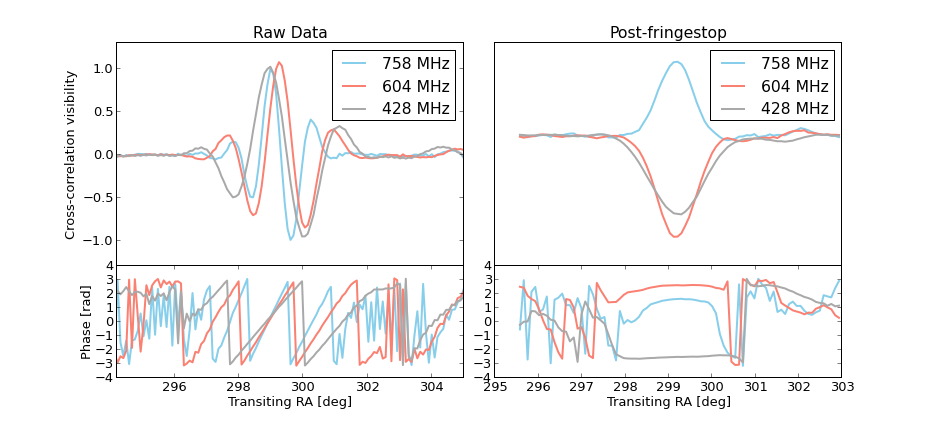
\includegraphics[trim={1in 0in 1in 1in}, width=\smwidth]{./figures/beamforming/thesis_fringestop.png}
\caption[abc]{An example of the fringestopping process that is 
 necessary for gain calibration off of a transiting point-source. Since 
 the phase of a visibility will have a time- and frequency-dependent 
 component, the measured correlation will fringe as the earth rotates in 
 a chromatic way. This effect can be removed by multiplying each visibility by 
 $e^{-i \phi_{m, n}(\rm t, \nu)}$, as determined by Eq.~\ref{eq-fringestop_phase}. 
 The top left panel shows the raw correlation between feeds 1 and 129 as a function of transiting
 $RA$, which are of the same polarization but 
 on opposite cylinders, separated by 21 m. We plot  
 three different frequencies. The panel below the top left
 shows the same complex visibility's phase. The slope, or fringe-rate, decreases 
 at lower frequencies, as expected. The right panel show the same data 
 after running it through the fringestopping pipeline. Though the resulting 
 phases are near flat, implying that the baseline is no long fringeing, 
 the visibilities are not purely real; this is because there are residual 
 instrumental phases. These phases can be solved for using an 
 eigendecomposition now that the array is phased up to a single point-source.}  
\end{center}
\end{figure}

% -------------------------------------------- FIGURE 1 --------------------------------------------


The visibilities we measure can be thought of as 
the upper triangle of an $N\times N$ complex Hermitian 
matrix, $\mathbf{V}$. This is simply the outer product of the 
signal vector, $\mathbf{x}$, with its Hermitian conjugate. 

\begin{align}
\label{eqn-corrmat}
\mathbf{V} = \mathbf{x} \mathbf{x}^\dagger &\approx \begin{pmatrix}
|g_0|^2\, e_0^2 &  & ... & & & \\ 
 &  &  & &  g_n g_m^* e_n e_m^*& \\ 
 &  &  \ddots & & & \\ 
 &  &  &  & & \\
&&&&&&\\
 &  &   &  & &  |g_N|^2 \, e_N^2
\end{pmatrix}
\end{align}
\\

If the sky is composed of a single point-source
then this matrix will be rank one, i.e. there is only one 
non-zero eigenvalue. One can see this by referring to Eq.~\ref{eqn-tsky} 
and noting that if the data has been fringestopped, then the phase 
component (which is different for each correlation) goes away and the 
sky temperature (which is the same) can be factored out of
Eq.~\ref{eqn-corrmat}, which becomes

\begin{equation}
\mathbf{V} = T(\mathbf{\hat{k}}) \, \mathbf{g} \mathbf{g}^\dagger.
\end{equation}

\noindent Therefore by diagonalizing the correlation matrix $\mathbf{V}$ 
we get a complex eigenvector corresponding to the largest 
eigenvalue, and that eigenvector is proportional to the gain vector $\mathbf{g}$. 
The phase of this eigenvector will be an estimate for the instrumental 
phases, $\phi_{g_n}$, up to some unknown global offset. The goodness 
of this calibration depends on the validity of our assumption 
that the correlation matrix is rank one. We can estimate the 
error on the calibration solution as the ratio of the second largest 
eigenvalue, $\lambda_2$, to the largest, $\lambda_1$. For typical 
frequencies we get values of $\frac{\lambda_2}{\lambda_1}\sim2\%$ 
when using Cyg A or Cas A.

These algorithms have been implemented in a pre-beamforming 
pipeline written in {\tt Python}. Every day a point-source transit 
is fringestopped and a calibration solution is solved for 
at each frequency.
The source chosen depends on the solar time of its transit: Since the
sun is extraordinarily bright in our band it will be in our side-lobes 
as long as it is above the horizon,
so the transit has to be 
at night for good calibration solutions. Historically, 
we have used Cygnus A in the spring and summer, Cassiopeia A 
in the summer and fall, and Tau A in the winter. 
Whatever we calibrate off of, the phases of that solution are 
written to pickle files that are then fed to the Pathfinder's FPGAs.
The FPGA then applies complex gains after channelization, which 
in theory should provide the beamforming kernel with voltages 
whose phases are purely geometric. 

\subsection{First coherent light}
Although the majority of the back-end was written within a couple  
of months, the beamformer required substantial 
on-sky testing and subsequent debugging. One important debugging tool 
came from utilizing the equivalence of the summed-and-squared
high-cadence data that was produced by the beamformer with the 
full $N^2$ integrated data. This is true because the correlation 
step does not erase any fundamental information about the electric field. 
The latter is nominally taken with $\sim21$ second
time samples for 32,896 correlation products coming from 256 feeds. 
The former is a sum over the feeds which can be integrated in time 
arbitrarily after squaring. Ignoring the time rebinning for a moment,
we can write the squared formed beam as,

\begin{align}
X_{\rm BF} X_{\rm BF}^* &= (w_1 x_1 + w_2 x_2 + ... + w_N x_N) (w_1 x_1 + w_2 x_2 + ... + w_N x_N)^*\\
&= |w_1|^2|x_1|^2 + ... + |w_N|^2|x_N|^2 + ... + w_1 w_2^* x_1 x_2^* + w_2 w_1^* x_2 x_1^* + ... , 
\end{align}

\noindent where, as before, $w_n$ are the 
complex weights applied in the beamformer 
and $x_n$ is a voltage stream from antenna $n$.
This can be rewritten as the sum of the 
auto correlations and twice the real part of the recorded 
phase-shifted cross-correlations.
\\

\begin{equation}
\label{eqn-bf_sum}
X_{\rm BF} X_{\rm BF}^* = \sum_{n\le N} |w_n|^2 V_{n, n} + 
2 \sum_{\substack{n,m\le N \\ n<m}} \Re e\{W_{n, m} V_{n, m}\}
\end{equation}
\\

In this equation we have let $W_{n, m} \equiv w_n w_m^*$.
Since the correlation matrix is Hermitian, its top 
and bottom triangles are redundant and one needs only to 
record $\frac{1}{2} N (N+1)$ of the $N^2$ pairwise products.
If we wrote all pairwise correlations, we would simply need 
to sum the correlation matrix after applying the relevant 
weights, i.e. summing after the Hadamard
product, $\mathbf{W} \circ \mathbf{V}$. This is identical 
to Eq.~\ref{eqn-bf_sum} if both matrices are Hermitian. 

Using the equivalence we have just described, one can compare the 
output of the beamformer to 
the $N^2$ visibilities after applying complex 
weights and summing the correlations. This is effectively 
off-line beamforming, though the cadence is too slow for 
the science goals of the real beamforming 
back-end, namely studying the time-variable sky. 
As a first test, 
we would form a stationary beam with only two feeds and let a 
bright point-source like Cas A drift through, 
producing a fringe pattern. We would then take 
the corresponding Cas A transit from the correlated ``cosmology" 
acquisition, using Eq.~\ref{eqn-bf_sum} and giving only non-zero 
weights to the two relevant feeds, and check if the two
fringe patterns were identical. We carried out a series 
of tests of escalating complexity, for example including more feeds in the sum, updating 
phases in real-time in order to track sources, and deliberately 
switching the weights with their conjugate to see if the fringe 
direction changed. Through these tests several bugs were discovered, 
including spherical trigonometry errors in the phase 
calculations and a disagreement between one piece of code's 
definition of $LST$. 

The final hurdle was more fundamental to CHIME's architecture,
though in principle it should not affect the cosmology experiment. 
It was found through 
early pulsar observations that the beamformer was only summing
coherently when the instrumental phases that are removed in 
the FPGAs are solved for with the lower-triangle of the correlation 
matrix. In other words, instrumental phases were not properly 
removed in the correlator unless they were applied as 
$e^{+i\phi_{g_n}}$ instead of $e^{-i\phi_{g_n}}$, as one would expect.
The perplexing thing was that in two years of analyzing 
the visibilities output by the correlator, nobody noticed a 
error in the sign-convention. And indeed, when we started to look
at the phase of the raw visibilities, we found the argument 
of an east-west baseline increases with time, which is 
what one expects from an upper-triangle correlator. This 
apparent paradox was solved by discovering \textit{two} sign 
reversals, one in the F-engine and one in the X-engine, that
effectively cancel each other out, but only if both are applied. 

Our digitizers sample at 800 MHz, taking advantage of the observing 
band between 400-800 MHz being in the second Nyquist zone.
However, when we channelize
the incoming time-stream data in the FPGAs, the complex conjugation 
associated with the aliased second Nyquist zone was not considered during the 
Fourier transform. Therefore the channelized voltages leave the F-engine 
with an opposite sign in the exponential. When they are correlated
in the X-engine it is also done in reverse order as, 

\begin{equation}
V_{n, m} = x_n^* x_m,
\end{equation}

\noindent as opposed to the upper-triangle correlation described by 
\citet{2015arXiv150306203K}, 

\begin{equation}
V_{n, m} = x_n x_m^*.
\end{equation}

The second sign convention error does not affect the beamformed 
output, since that data stream is never correlated. We therefore 
needed to account for this for the back-end to work. An example 
of an early verification of the beamformer's sign convention 
and the first successful tracking observation is shown in Fig.~\ref{fig-bf_b0329}. 
The collaboration has decided to keep these sign conventions as is
and make note of it going forward, rather than re-write any low-level 
software.


\begin{figure}[!h]
\label{fig-bf_b0329}
\begin{center}
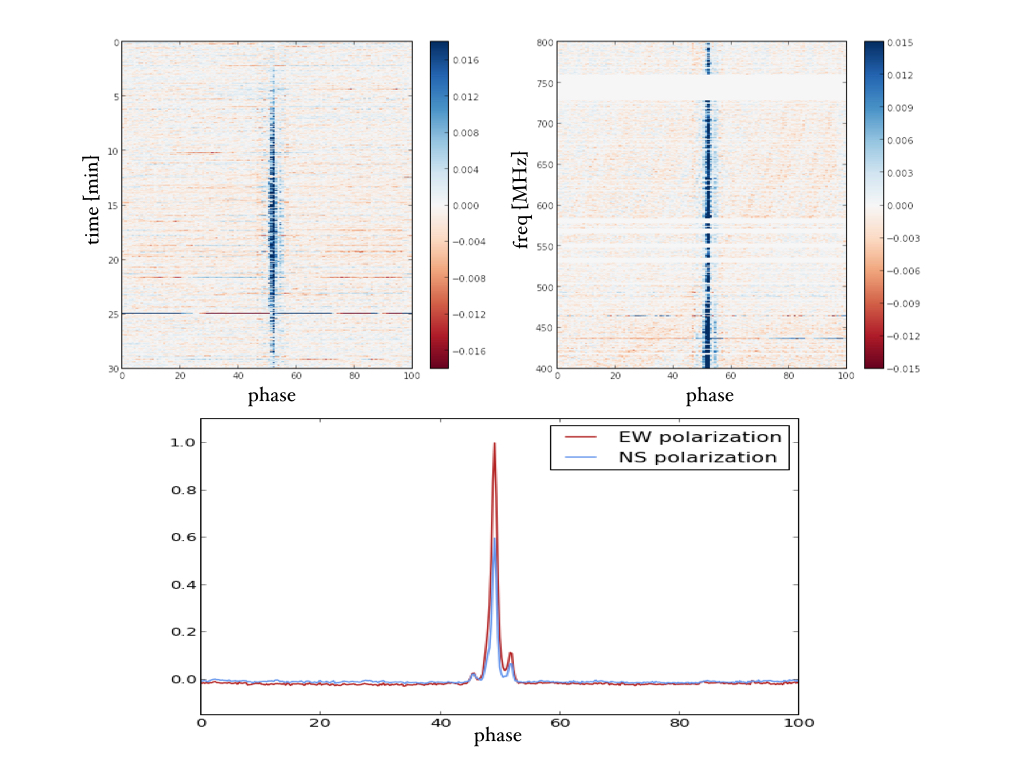
\includegraphics[trim={0.8in, 0in, 0in, 0in}, scale=0.5]{./figures/beamforming/b0329_testing.jpeg}
%\vspace{0.0cm}
\caption[abc]{First coherent pulsar observations with CHIME. This 
brief observation of B0329+54 provided us with an idea 
of the instrument's sensitivity and polarization response. 
Perhaps more significantly, it taught us that 
that our X-engine is a lower-triangle correlator, rather than 
upper-triangle like we thought, and that our F-engine \textit{also}
conjugates with the opposite sign. \textit{top left:} waterfall plot
of the pulsar's Stokes I profile over the $\sim$30 minutes when the 
source enters then exits our beam. \textit{top right:} frequency 
vs. phase Stokes I, integrated over roughly 15 minutes. 
\textit{bottom:} time- and frequency-averaged pulse profile 
for the two polarizations autocorrelations. The difference between 
the east-west and north-south beams give an estimate for Stokes Q, which 
includes both intrinsic polarization ($\sim10\%$ for this source)
and instrumental leakage.} 
\vspace{0.4cm}   
\end{center}
\end{figure}


\section{FRB VLBI search}
\label{vlbi_frb}

In 1967 Canada achieved an historic feat by doing 
the first ever successful VLBI observation. The fringes were 
obtained between DRAO and ARO, with a baseline of 3,074 km \citep{1967Natur.215...38B}. 
This result was given a ``Milestone'' award from 
The Institute of Electrical and Electronics Engineers (IEEE), 
which was also awarded for the inception of the Internet, transmission 
of transatlantic radio signals, and the discovery of Maxwell's equations \citep{IEEEmilestone}. 
We have attempted to recreate the same VLBI baseline, but instead of 
using the considerable spatial resolution on quasars as in 1967, 
we are attempting to localize FRBs. 


\subsection{Motivation}

The CHIME Pathfinder is meant to have only one synthetic beam. 
Its purpose is primarily to act as a test-bed for the more powerful 
pulsar and FRB back-ends that will be attached to the 
full four-cylinder CHIME. However since the Pathfinder is on 
sky at all times and the beamformer we have built does not 
interrupt the ongoing cosmology acquisition, we decided to 
build a preliminary FRB search. We also have as many as three 
other telescopes onto which we can mount 
CHIME feeds and observe in our band: the Algonquin Radio Observatory (ARO), 
the John A. Galt 26m, and the Green Bank 140ft telescope. This would
allow for the first ever VLBI detection of an FRB. 

This is interesting for a few reasons. From a development 
standpoint it allows us to understand better various stages of the 
CHIME-FRB pipeline, including the rate of 
RFI false-positives, our algorithm's search 
efficiency, and specs on the regularity and precision of instrumental 
gain removal. It will also give us a good sense of how the real CHIME 
beams behave on the sky. Perhaps most interestingly, 
we could reasonably expect to see a burst after several months of 
observing, hopefully in coincidence with the telescopes previously mentioned. 
We could therefore not only detect an FRB with sub-arcsecond resolution,
but also would the first source in our band, at 400-800 MHz, 
including full polarization information. While searching 
for fast radio bursts, we could also find RRATs and new slow pulsars, since 
a significant fraction of the Galaxy transits each day.

\subsection{Implementation}

We have had a working beamforming back-end on the CHIME 
Pathfinder since October 2015. It has been used primarily 
for short tracking pulsar observations, but had stability issues 
on timescales of $\sim$days, meaning we could not run it 
for long periods without interfering with the regular cosmology acquisition. 
However in the past several months a number of new features 
were added that allow not only long-term beamforming captures, 
but also transient searching. 
 
A real-time, multithreaded acquisition code that takes in the VDIF 
packets coming out of the X-engine, and rearranges them to either be written to disk or search for 
FRBs\footnote{https://github.com/kmsmith137/ch\_vdif\_assembler}. Attached 
to this packet reader was a tree-dedispersion search code, some of 
which had been used before on Green Bank 100m data and a real-time ARO 
search\footnote{https://github.com/kiyo-masui/burst\_search}.
The CHIME acquisition software {\tt kotekan} was 
altered in a number of ways, fixing the long-term 
stability issues in the beamforming kernel. These systems 
were synthesized into a real-time transient search back-end 
that has been on sky since May 2016. 
It is outlined in Fig.~\ref{fig-bf_diagram}
on page \pageref{fig-bf_diagram}. 

Since CHIME is a transit telescope with a long north-south beam, 
our formed beam is effectively confined to the meridian. This means
we must choose an optimal declination on which 
to park the beam. As a sanity check, we spent $\sim10$ 
days pointed 
at the declination of pulsar B0329+54, which is the 
brightest switching source in the northern sky in our band. It 
is dispersed with 26.833 pc cm$^{-3}$ and its individual 
pulses are bright enough to detect, meaning our tree-dedispersion 
algorithm ought to find its individual pulses. The search 
algorithm looks at time blocks of 100 seconds, searches 
for DMs between 10-2000 pc cm$^{-3}$ with widths between 
1-100 ms, and looks for peaks above 8$\sigma$. If it finds something
it ``triggers'' and writes out an image file containing the peak 
in DM / arrival time space, a dedispersed waterfall plot, a dedispersed 
pulse profile, and a fluence frequency spectrum. An example 
of the B0329+54 is shown in Fig.\ref{fig-b0329_trigger}. It also 
writes {\tt numpy} arrays containing the squared and summed 
intensity data. It then moves on to the next block of 100 seconds, 
overlapping with the previous one by 18 seconds. 


\begin{figure}[!h]
\label{fig-b0329_trigger}
\begin{center}
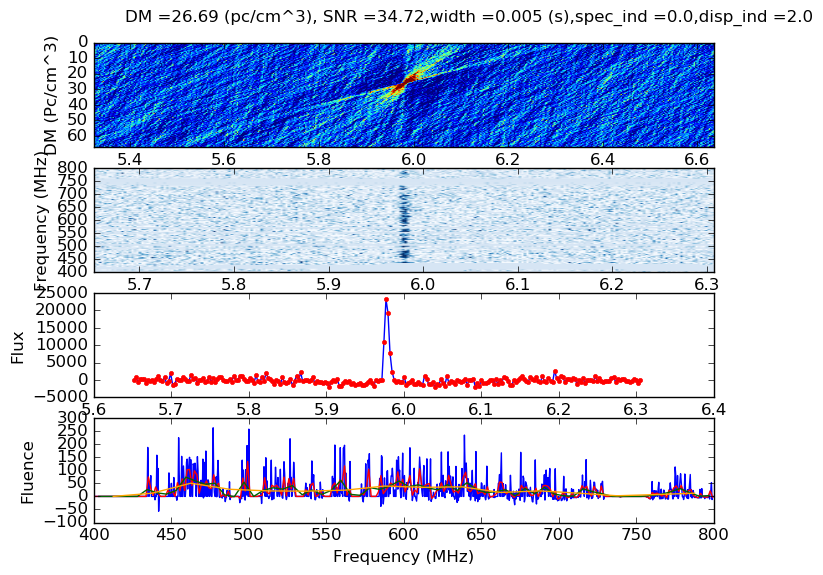
\includegraphics[trim={0in, 0in, 0in, 0in}, scale=0.75]{./figures/beamforming/b0329_trigger.png}
\caption[abc]{Example of a figure created after a trigger 
on the Pathfinder FRB search. This trigger was during the transit of 
pulsar B0329+54, on whose declination our synthetic beam was 
parked. Further information about the pulse is 
included at the top of the figure, including 
signal-to-noise ratio, width, and dispersion index. Though the 
beam is not well calibrated in absolute flux, this pulsar 
is of order 10 Jy, so this pulse might be half as bright 
as the original Lorimer burst \citep{lorimer-2007}. 
\textit{Top panel:} The search results 
in dispersion measure vs. arrival time space. The red, butterfly-like 
cluster of points around DM of 25 pc cm$^{-3}$ and arrival time 
6 seconds into the 100 second block, 
shows the detection of a single B0329+54 pulse. 
\textit{Second panel:} A frequency 
vs. time colour map showing the dedispersed pulse. \textit{Third panel:} 
Pulse profile for this trigger, averaged over frequency after 
masking RFI and weighting by inverse system temperature. \textit{Bottom panel:}
Fluence vs. frequency plot of the pulse.}  
\vspace{0.4cm}   
\end{center}
\end{figure}

\subsection{ARO FRB search}




\begin{figure}[!h]
\label{fig-bf_diagram}
\begin{center}
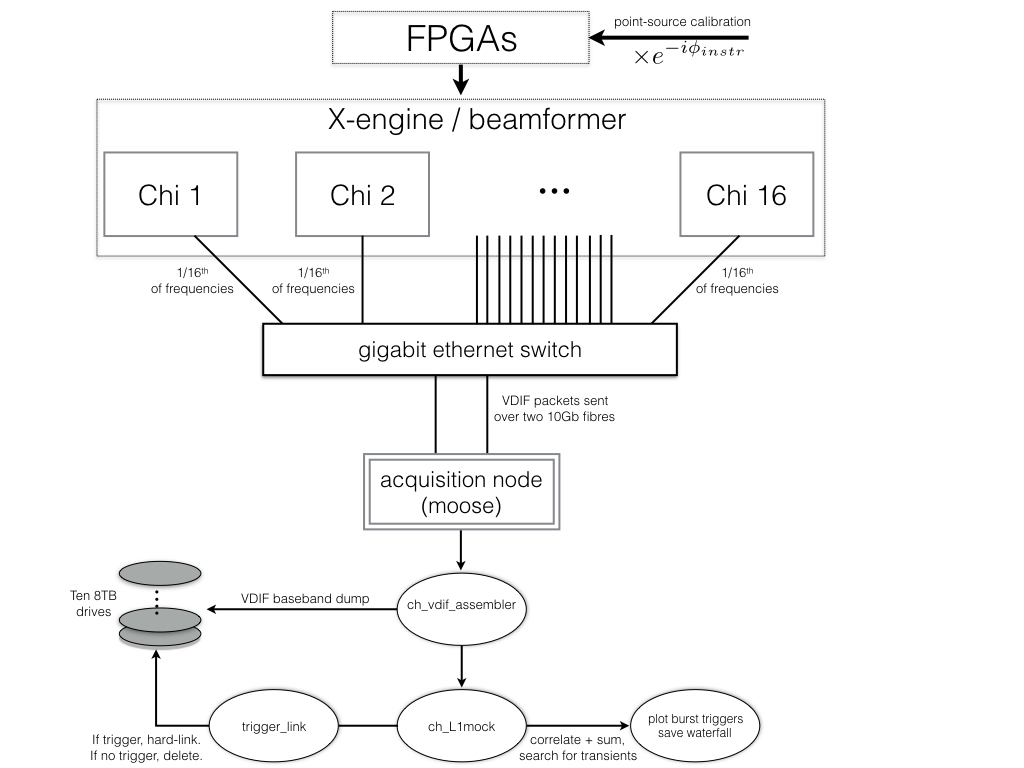
\includegraphics[trim={1.in, 0in, 2.5in, 0in}, width=1\textwidth]{./figures/beamforming/moose_diagram.png} 
%\vspace{0.0cm}
\caption[abc]{Block diagram of the beamforming back-end on CHIME Pathfinder. 
A calibration solution is obtained from a bright point-source transit, 
the phases of which are fed into the FPGAs where they are applied as a 
digital gain. All antenna signals are then sent the $X$-engine, 
comprised of 16 GPU nodes. Each node applies geometric phases then 
sums the voltage stream across all antennas with the same polarization. 
The two resultant beams are then sent to our acquisition machine {\tt moose} 
as {\tt VDIF} packets, where a multi-threaded capture code, {\tt ch\_vdif\_assembler}. 
At this point the baseband data are either written to disk as scrambled baseband 
{\tt VDIF}, or they are reorganized in time and frequency. The ordered data are 
searched for FRBs after squaring and integrating to $\sim$millisecond cadence 
using a tree-dedispersion algorithm. If there is a trigger, then the corresponding 
baseband data is hard-linked. Old files that haven't been hard-linked are deleted
periodically.}
\end{center}
\end{figure}

\subsection{Results}
As we discuss in chapter \ref{chapter:frb_statistics}, there is 
a large uncertainty in the FRB rate between 400-800 MHz. There 
is even greater uncertainty in the expected rate for a 
telescope like the CHIME Pathfinder. This is because at the moment of 
this thesis all FRBs
have been detected with large-collecting area, highly sensitive single-dish 
telescopes (GBT, Parkes, and Arecibo). Therefore in order to 
extrapolate the rate estimates on to the Pathfinder, which 
does not have much collecting area and whose beam is quite large, one 
needs to know the underlying flux distribution. As we will show 
in Eq.~\ref{eq-sensitivity_rat}, the rate depends on the product 
of the telescope's field-of-view (FoV) and a thermal sensitivity term. 
This scales $\propto A^{-1} A^\gamma$, where $A$ is collecting area 
and $\gamma$ is the FRB flux distribution's power-law index, which is 
$3/2$ if FRBs are non-cosmological and Euclidean. If $\gamma < 1$, 
as is expected in the cosmological FRB scenario, then 
small telescopes are actually advantageous over large single-pixel telescopes 
since the beamsize becomes more important. 

With a dish like the Pathfinder
the rate is roughly 10 times higher if $\gamma\approx 0.8$ (cosmological scenario) 
compared to the Euclidean scenario. This is because its relatively 
low sensitivity per steradian requires there be large numbers 
of very bright bursts, which one gets from a flat distribution.

\subsection{False positives}

Most transient searches are plagued by non-celestial sources masquerading 
as astronomical events. In the case of dedispersion searches on 
radio telescopes, these can be caused by RFI, numerical relics 
in the signal chain, or statistical fluctuations. 
At UTMOST, \citet{2016MNRAS.458..718C} found 
10$^2$ events per hour in transit mode across all beams. \citet{2015MNRAS.451.3933P}
found the source of an elusive but persistent set of triggers 
to be due to an on-site microwave oven's magnetron shutdown phase. These 
``Perytons" are unique in their conspiratorial ability to 
look like a real burst, but they are a subset of a broader zoo 
of RFI-induced false triggers. 

At DRAO, although the region is officially 
protected from radio contamination, about 15$\%$ of the CHIME
band is presently lost to RFI (see the bottom left 
panel of Fig.~\ref{fig-lte_trigger}). Recently, Rogers Communications 
paid several billion Canadian dollars for a 700 MHz 
Long-Term Evolution (LTE) band for cellphone service.
Unlike the satellite television 
stations that we see at 500-600 MHz, the LTE band 
fluctuates on timescales of milliseconds to seconds, which can affect 
a millisecond transient search. Fig.~\ref{fig-lte_trigger} shows 
an example of this RFI false positive from the LTE band. 

%trim={<left> <lower> <right> <upper>}
\begin{figure}[!h]
\label{fig-lte_trigger}
\begin{center}
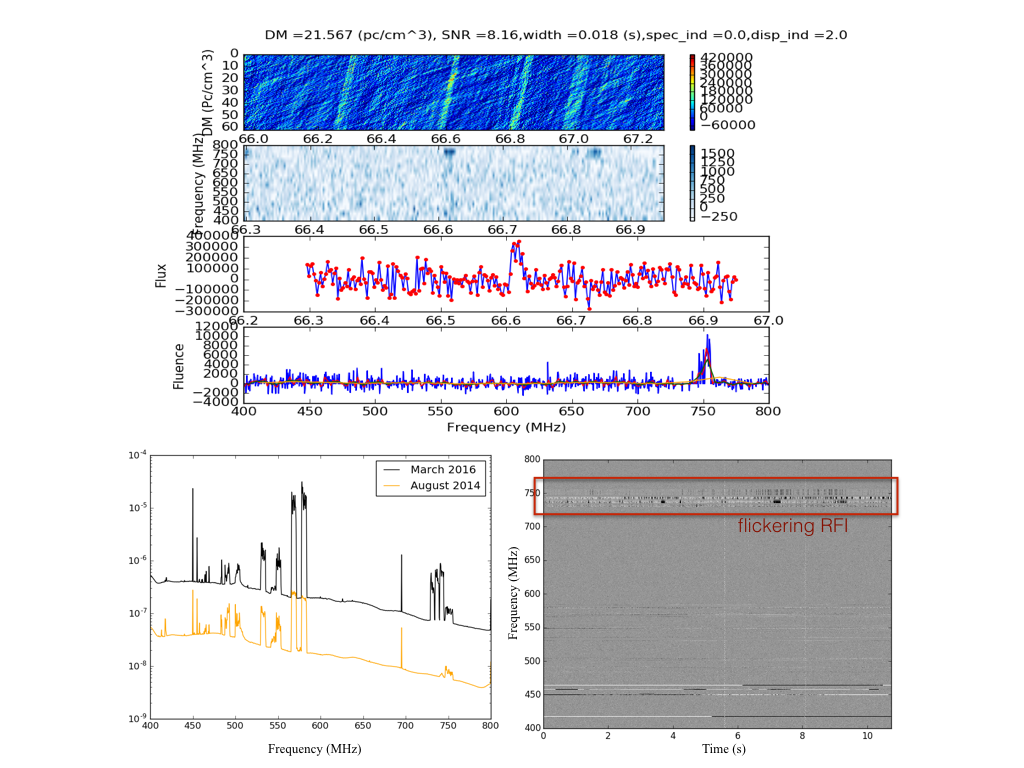
\includegraphics[trim={0in 0in 0in 0in}, scale=0.5]
{./figures/beamforming/lte_trigger.png}
\vspace{0.0cm}
\caption[abc]{A false positive trigger caused by the flickering 
LTE band that, the likes of which 
caused $\sim$90$\%$ of the alerts before it was removed.
It is of course simple to reject; one can just mask 
out the relevant channels.
However, it provides a useful example of the types of 
short-timescale RFI that can affect an FRB survey.}
\end{center}
\end{figure}



\section{Conclusion}
\label{sec:conclusion}
  

% ================================================================================
% ACKNOWLEDGEMENTS
% ================================================================================


  
